

\documentclass{report}

\usepackage[tc]{titlepic}
\usepackage[utf8x]{inputenc}
\usepackage[french]{babel}
\usepackage{graphicx}
\usepackage{geometry}
\usepackage{ifthen}
\usepackage{enumerate}

\graphicspath{{fig/}}

\newcommand\Titre{Devoir 1}
\newcommand\Auteur{Maxence Caron, Jules Caron, Hugues Soares}
\newcommand\Destinataire{Ronald Beaubrun}
\newcommand\NomEquipe{GLO-2000}
\newcommand\DateRemise{\today}


\geometry{letterpaper,%
          centering,%
          hmargin={2.5cm,2.5cm},%
          vmargin={2.5cm,2.5cm},%
          heightrounded,%
	  includehead}


\newenvironment{thebibliographyUL}[1]%
               {\clearpage%
                \begin{thebibliography}{#1}%
                \addcontentsline{toc}{chapter}{\bibname}%
                \raggedright%
               }%
               {\end{thebibliography}}

\renewcommand\maketitle{
	\thispagestyle{empty}%
	\pagenumbering{roman}%
	\begin{titlepage}%
		\setcounter{page}{999}%
		\begin{flushleft}
			
\includegraphics[width=12em]{ul_logo}
		\end{flushleft}\par
		\vspace*{\stretch{1}}
			\centering
			\parbox{\textwidth}{\centering\Large\bfseries \Titre}         \\[5ex]
			\vspace*{\stretch{2}}
			pr\'{e}sent\'{e} \`{a}                    \\[1ex]
			\textbf{\Destinataire}                 \\
			\vspace*{\stretch{1}}
		par                                       \\[1ex]
			{\large \'{E}quipe \NomEquipe}                \\[1ex]
			\Auteur\\[1ex]
			\vspace*{\stretch{1}}
			{\large Universit\'{e} Laval}             \\
			\DateRemise\\
	\end{titlepage}
}

% Definition du niveau hierarchique maximum couvert par la table des matieres
\setcounter{tocdepth}{3}            % default = 2

% Definition du niveau hierarchique maximum ayant une numerotation
\setcounter{secnumdepth}{3}         % default = 2

\begin{document}

\maketitle
%\tableofcontents
%		\ifthenelse{\boolean{false}}%
%			{\clearpage%
%			\listoffigures%
%			\addcontentsline{toc}{chapter}{\listfigurename}}{}
%		\ifthenelse{\boolean{false}}%
%			{\clearpage%
%			\listoftables%
%			\addcontentsline{toc}{chapter}{\listtablename}}{}

\cleardoublepage%
\setcounter{page}{1}%
\pagenumbering{arabic}%

\chapter{Réseaux - lab 1}


\section{Question 1}
\begin{enumerate}[(a)]
	\item 
		\[ P(\%) = f(m, p, h_1, h_2, h_3) = 
		\frac{m}{\frac{8*2p}{3}h_1 + \frac{8*p}{6}h_2 + \frac{8*p}{6}h_3 + m)} 100\%\]
	
	\item 
		En assumant que le meme nombre de couches qui ajoutent $h_3$ reste le même qu'à la
		question a) :
		\[ P(\%) = f(m, p, h_1, h_2, h_3, h_4) = 
		\frac{m}{\frac{8*2p}{3}h_1 + \frac{8*p}{6}h_2 + \frac{8*p}{6}h_3 + \frac{8*p}{6}h_4 + m)} 100\%\]
	En assumant que le nombre de couches qui ajoutent $h_3$ est le nombre de couches restantes :  
		\[ P(\%) = f(m, p, h_1, h_2, h_3, h_4) = 
		\frac{m}{\frac{8*2p}{3}h_1 + \frac{8*p}{6}h_2 + 0h_3 + \frac{8*p}{6}h_4 + m)} 100\%\]
	\item
		\[ P(\%) = f(16000, 6, 128, 256, 0, 64) = 
		\frac{16000}{\frac{8*2*6}{3}128 + \frac{8*6}{6}256 + \frac{8*6}{6}64 + 16000)} 100\% = 70.62\%\]
\end{enumerate}

\section{Question 2A}

\begin{enumerate}[(a)]
	\item
		\vspace{10mm}
		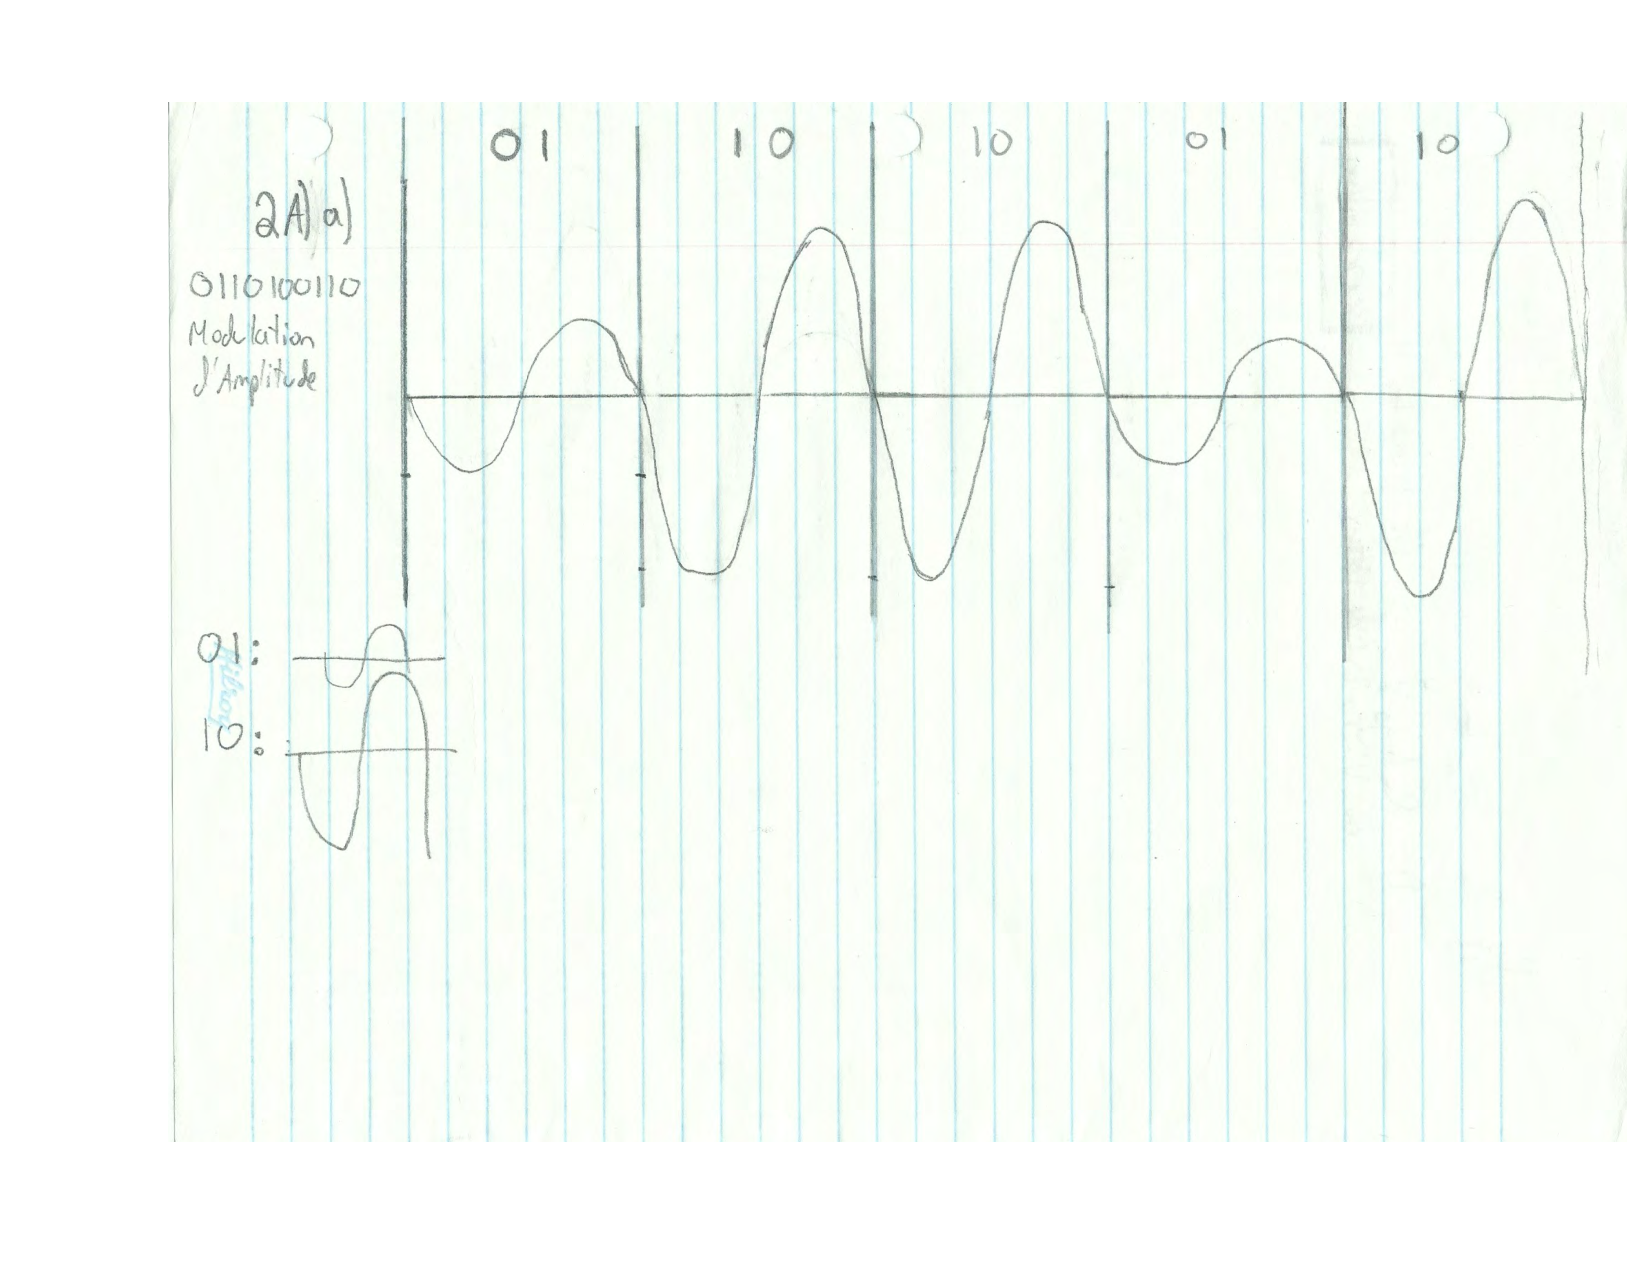
\includegraphics[page=1,scale=0.5]{julesScan}
	\item 
		\includegraphics[page=2,scale=0.5]{julesScan}

\end{enumerate}

\pagebreak

\section{Question 2B}

\begin{enumerate}[(a)]
	\item 
		\[R_m = 1500\]
		\[D = R_m\log_2 V = 1500\log_2 4 = 3000bits/sec\]
		Ou $V$ est égale au nombre de valeurs
	\item 
		\includegraphics[page=4,scale=0.5]{julesScan}
		
\end{enumerate}

\section{Question3}

\begin{enumerate}[(a)]
	\item 
		\includegraphics[page=5,scale=0.5]{julesScan}
	\item 
		\includegraphics[page=6,scale=0.5]{julesScan}
\end{enumerate}

%stuff

\section{Question 4}
\begin{enumerate}[(a)]
	\item 
		utilisation max du canal = $\frac{1000 bits}{2 * 0.250s} = 2000\frac{bits}{s}$
	\item
		$W = 2^n-1 = 2^(3bits)-1 = 7 trames$\\
		utilisation max du canal = $\frac{7 * 1000 bits}{2 * 0.250s} = 14000\frac{bits}{s}$
	\item
		$W = 2^n-1 = 2^(3bits)-1 = 7 trames$\\
		utilisation max du canal = $\frac{7 * 1000 bits}{2 * 0.250s} = 14000\frac{bits}{s}$
\end{enumerate}

% 1 mbps = 1M bits per sec
% delais 250ms
% trame 1000 bits, taille entete = 0,
% canaux codes sur 3 bits


\end{document}

